%\documentclass{article}
\documentclass[UTF8]{ctexart}
% Language setting
% Replace `english' with e.g. `spanish' to change the document language
\usepackage{gensymb}
\usepackage[english]{babel}
\usepackage{graphicx}
\usepackage{float}
\usepackage{subfigure}
% Set page size and margins
% Replace `letterpaper' with `a4paper' for UK/EU standard size
\usepackage[a4paper,top=2cm,bottom=2cm,left=3cm,right=3cm,marginparwidth=1.75cm]{geometry}

% Useful packages
\usepackage{amsmath}
\usepackage{graphicx}
\usepackage[colorlinks=true, allcolors=blue]{hyperref}

\title{搭建衍射光谱仪}
\author{BrightMoon}

\begin{document}
\maketitle
\section{设计思路}
总体设计的示意图和实物图参见图\ref{光谱仪}。
\subsection{理论基础}
利用光通过衍射光栅发生衍射,且不同波长的光衍射光斑位置不同的性质,把不同波长的光区分开。这里主要参考的是夫琅禾费衍射,相关光路图见图\ref{Fig.sub.1}。
\begin{figure}
\centering  %图片全局居中
\subfigure[夫琅禾费衍射光路图:入射光垂直于光栅AB;衍射光大角度斜射光屏。]{
\label{Fig.sub.1}
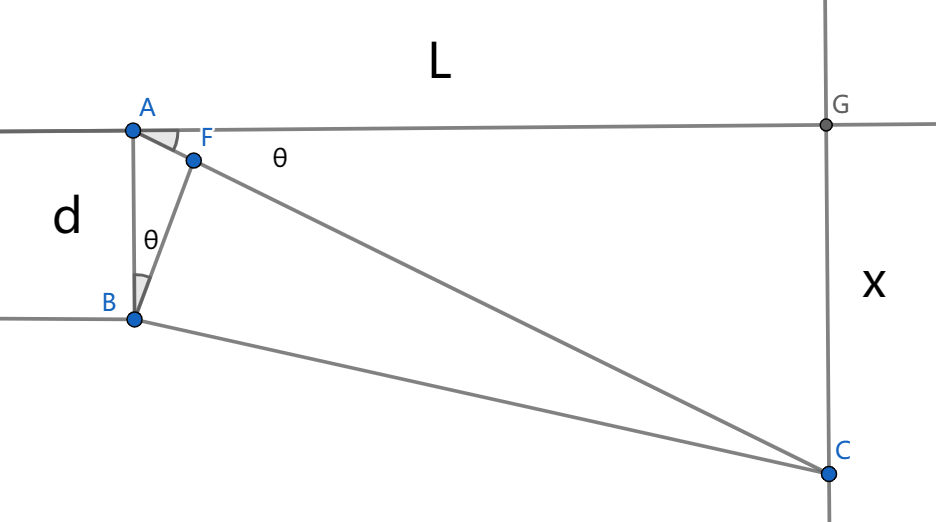
\includegraphics[width=7cm,height = 3cm]{夫琅禾费衍射.png}}
\subfigure[改进的衍射光路图:入射光斜射光栅;衍射光小角度斜射光屏。]{
\label{Fig.sub.2}
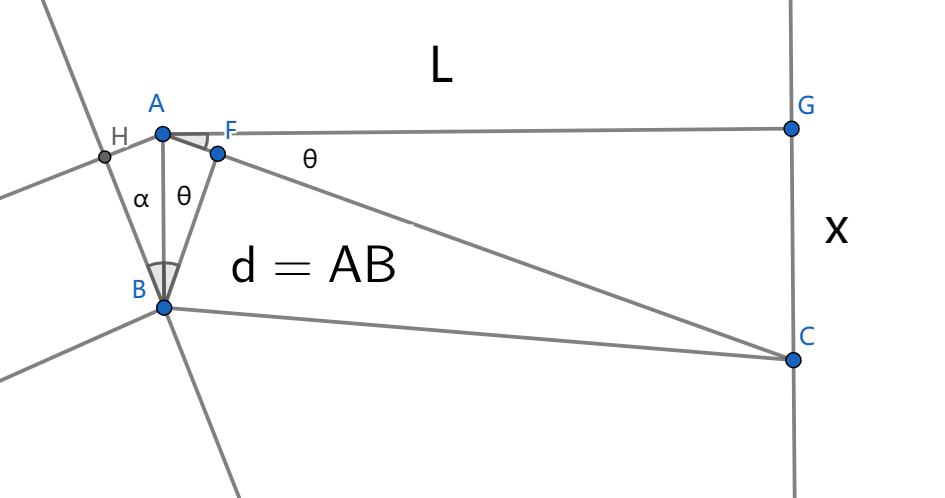
\includegraphics[width=7cm,height = 3cm]{改进的光路.png}}
\caption{衍射光路图示意:其中AB代表光栅,GC代表光屏;$\alpha$代表入射角,$\theta$代表衍射角。}
\label{光路示意}
\end{figure}
\subsection{重要改进}
\subsubsection{使用纯粹夫琅禾费衍射潜在的问题}
\begin{align}
    &d\sin \theta = \lambda\\
    &\theta \approx \sin \theta = \frac{\lambda}{d}\approx \frac{700\ nm}{10^{-3}\ mm}=0.7\ rad=40\degree
\end{align}

夫琅禾费衍射要求入射光垂直于光栅与光屏,光栅与光屏平行放置。这样造成的结果就是,衍射光线\textbf{以较大角度}斜向打在光屏上。然而,我们知道,用摄像头充当光屏的最大问题在于,\textbf{镜头存在视角$\gamma$}。而我所使用的摄像头视角比较小($\gamma \approx 30\degree$),利用\textbf{这种方法不能完整接收所有可见光波段的衍射光}。
\subsubsection{改进方案}
于是,我想到,可以让入射光斜射光栅,这样,在通过衍射光栅之前,就已经产生了光程差,使得衍射光线接近于垂直的方式,小角度斜射光屏,从而可以被手机镜头完整接收到(图\ref{Fig.sub.2})。
\begin{align}
    &d\sin \alpha +d\sin \theta = \lambda,\quad \text{令}\alpha \approx 45\degree\\
    &|\theta |\approx |\sin \theta| = |\frac{\lambda}{d}-\sin \alpha |\approx |\frac{700\ nm}{10^{-3}\ mm}-\frac{\sqrt{2}}{2}|=4.5\degree
\end{align}
并且这种方式下,不同波长的光的一级衍射明纹,在光屏上近似线性分布($x$是$\lambda$的一次函数)。
\[x=L\tan \theta  \approx L\sin \theta  = L(\frac{\lambda}{d}-\sin \alpha )\]
\[\frac{\Delta x}{\Delta \lambda}\approx \frac{L}{d}\]
\subsubsection{编写程序}
在相机的CMOS上,光谱彩带只占很小一个区域,为了简明清晰,需要将这一区域截取而丢弃其它部分。对于这条光谱彩带,我需要分析各处的相对光强,这里需要图像处理,得到每一纵列像素的平均灰度值(表示光强)。然后需要把这一组数据可视化成柱状图。为了操作简便,我编写了一个Python程序,用来一次性实现下述功能:
\begin{enumerate}
    \item 拍照并裁剪画面(裁剪区域作为一个重要参数,\textbf{首次使用}需要通过实验确定)。
    \item 标定横轴(不同位置对应何种波长,\textbf{首次使用}需要在实验中用红绿激光校准)。
    \item 计算相对光强(相对灰度值)并绘制相对光强对不同波长$\lambda$(位置$x$)的柱状图。
\end{enumerate}
\begin{figure}
\centering  %图片全局居中
\subfigure[设计示意图]{
\label{Fig.sub.3}
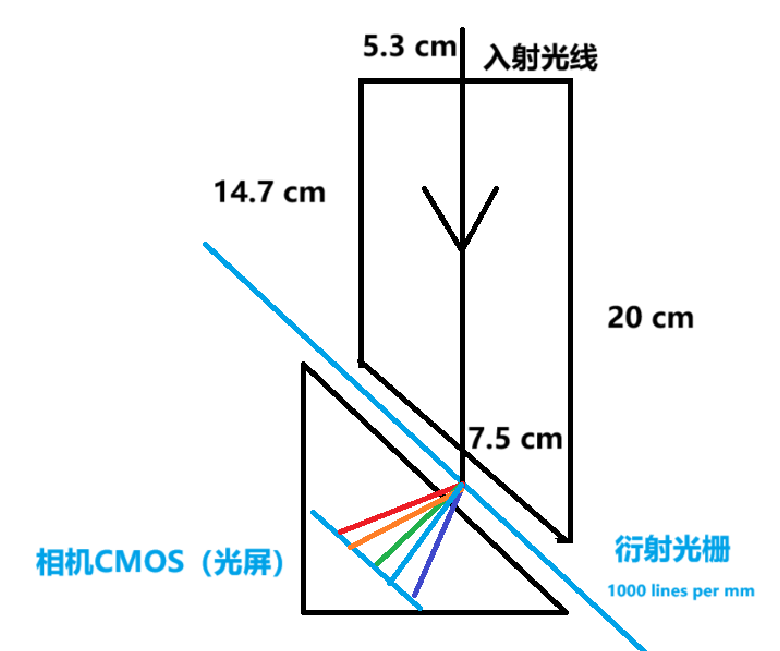
\includegraphics[width=7cm,height = 5cm]{设计图.png}}
\subfigure[实物图]{
\label{Fig.sub.4}
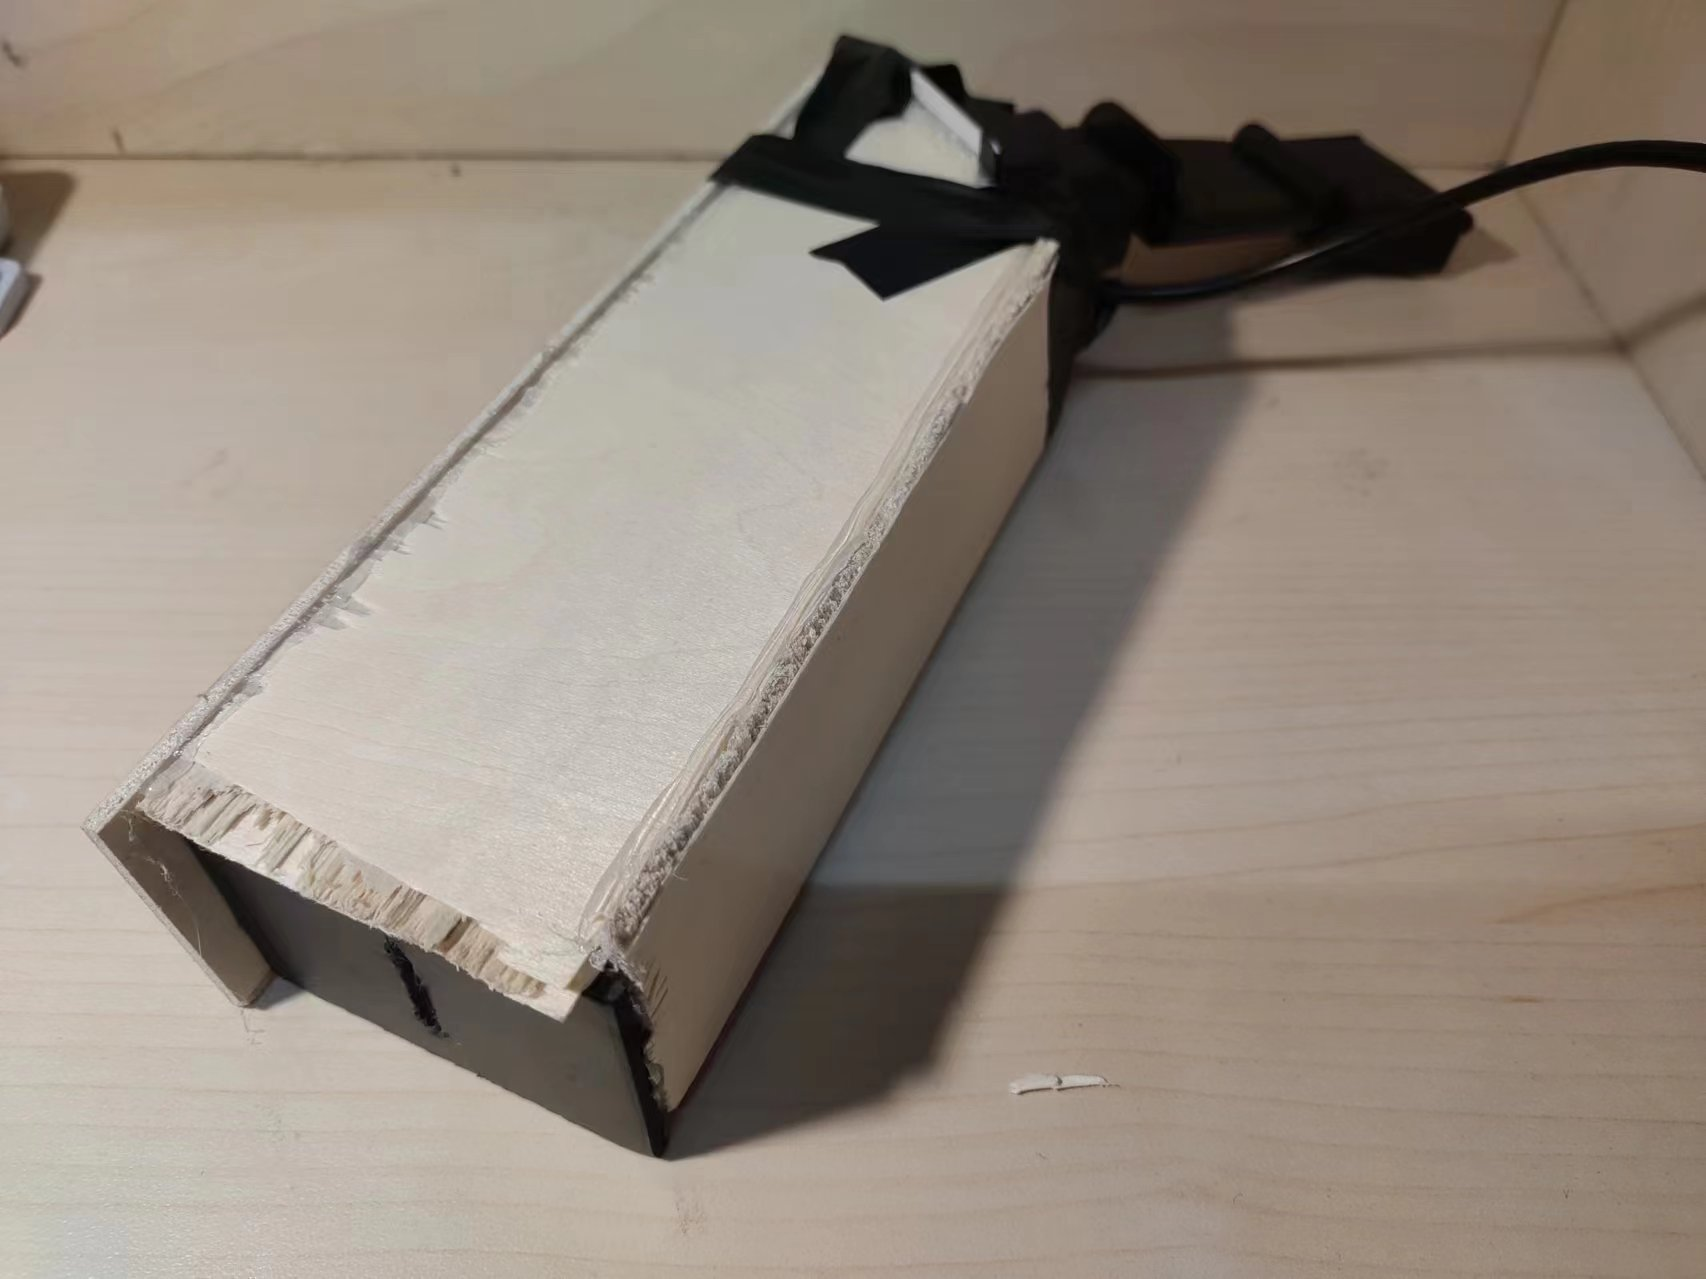
\includegraphics[width=7cm,height = 5cm]{实物图.jpg}}
\caption{我设计的衍射光谱仪}
\label{光谱仪}
\end{figure}
\section{使用时的操作步骤}
\begin{enumerate}
    \item 确定裁剪区域,只保留包含色带的窄长条。
(这是一劳永逸的测量,对于同一个机械装置,一旦确定,以后使用无需重复)
    \begin{enumerate}
        \item 确定横向两端边界。\textbf{本装置为[350,620]水平像素区间。}
        \item 确定纵向两端边界。\textbf{本装置为[190,210]垂直像素区间}
        \item 输入程序,\textbf{而后保持不变}。
    \end{enumerate}
    \item 标定基准波长,利用红绿两种激光。(\textbf{在经过裁剪的画面中})
    (这是一劳永逸的测量,对于同一个机械装置,一旦确定,以后使用无需重复)
    \begin{enumerate}
        \item 确定红色激光对应的横向坐标。\textbf{本装置为34.8水平像素坐标,对应650nm红色激光。}参考图\ref{Fig.sub.5}
        \item 确定绿色激光对应的横向坐标。\textbf{本装置为137水平像素坐标,对应532nm绿色激光。}参考图\ref{Fig.sub.6}
        \item 输入程序,而后保持不变。
    \end{enumerate}
    \item 再进行无数次测量。
    \begin{enumerate}
        \item 不需要再调整任何参数,只需要反复运行程序即可。
    \end{enumerate}


\end{enumerate}
\begin{figure}
\centering  %图片全局居中
\subfigure[红色激光校准:34.8水平像素坐标对应650nm波长]{
\label{Fig.sub.5}
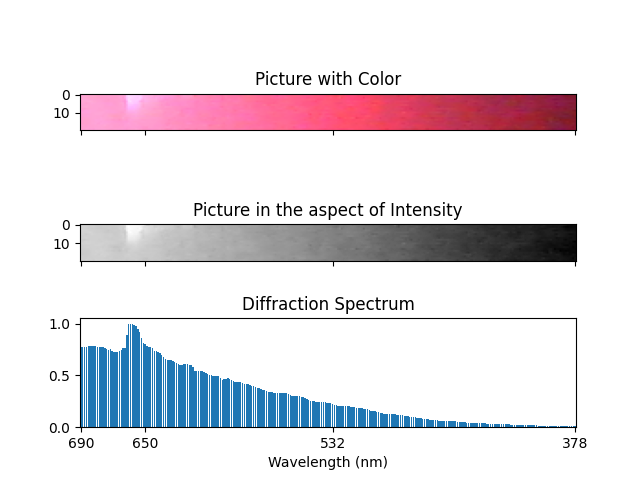
\includegraphics[width=7cm,height = 5cm]{红色激光.png}}
\subfigure[绿色激光校准:137水平像素坐标对应532nm波长]{
\label{Fig.sub.6}
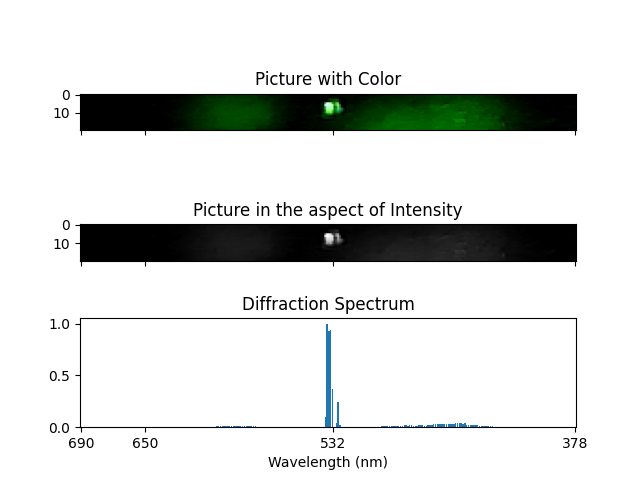
\includegraphics[width=7cm,height = 5cm]{绿色激光.png}}
\caption{激光校准过程}
\label{激光校准过程}
\end{figure}

\section{观测结果}
我以图片的方式,展示观测结果。日光以及接近日光的光源参见图\ref{日光以及接近日光的光源};LED光源参加图\ref{不同颜色的LED}。
\begin{figure}
\centering  %图片全局居中
\subfigure[日光:波段较宽而且连续]{
\label{Fig.sub.7}
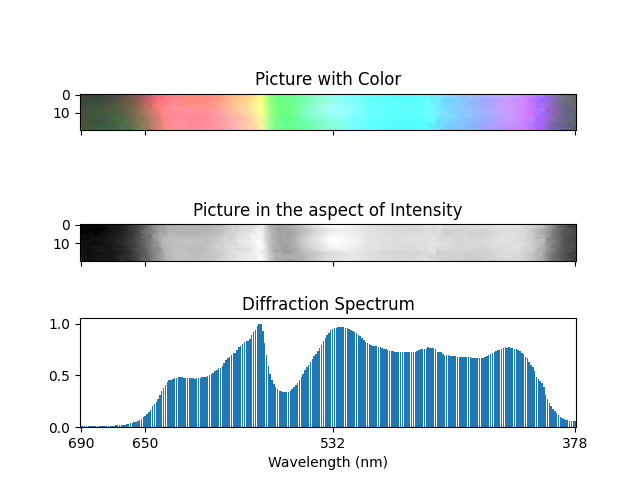
\includegraphics[width=4cm,height = 3cm]{日光16_29.png}}
\subfigure[教室大灯]{
\label{Fig.sub.8}
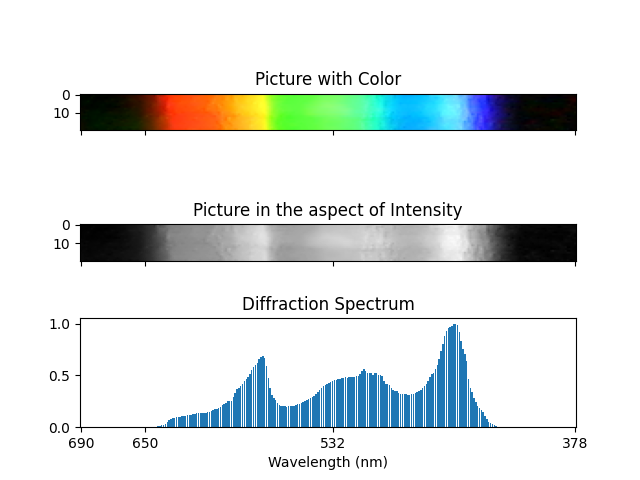
\includegraphics[width=4cm,height = 3cm]{教室大灯.png}}
\subfigure[我的台灯]{
\label{Fig.sub.9}
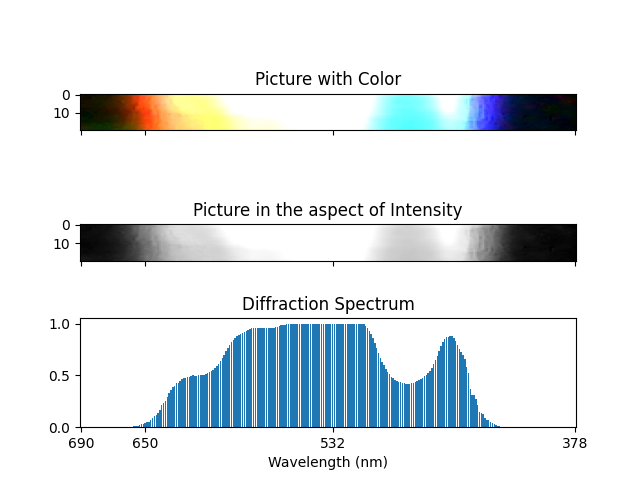
\includegraphics[width=4cm,height = 3cm]{我的台灯.png}}
\subfigure[我的手机]{
\label{Fig.sub.10}
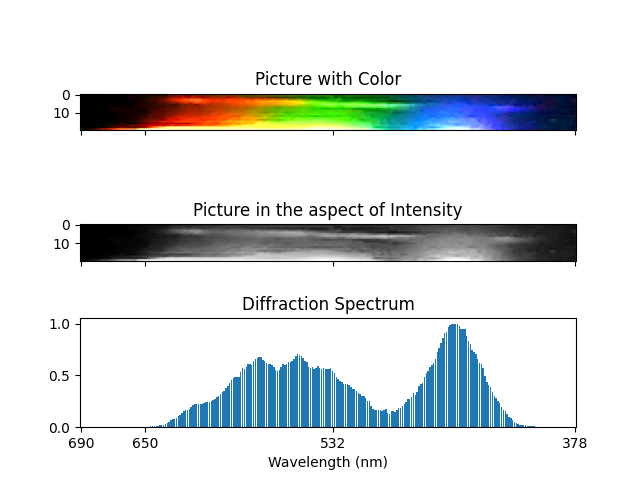
\includegraphics[width=4cm,height = 3cm]{我的手机IQOO U!.png}}
\subfigure[宿舍荧光灯:有明显的分立光谱]{
\label{Fig.sub.17}
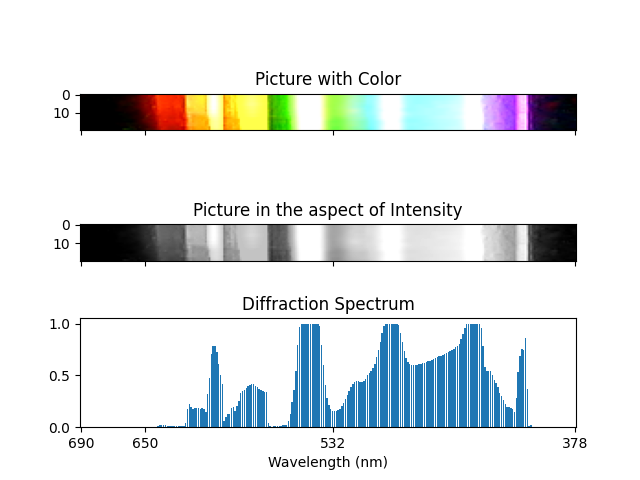
\includegraphics[width=4cm,height = 3cm]{宿舍荧光灯3.png}}
\caption{日光与接近日光的光源}
\label{日光以及接近日光的光源}
\end{figure}


\begin{figure}
\centering  %图片全局居中
\subfigure[红色LED]{
\label{Fig.sub.11}
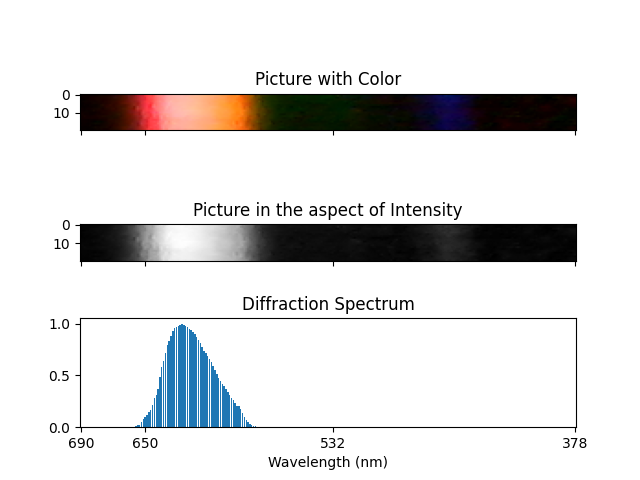
\includegraphics[width=4cm,height = 3cm]{红色LED.png}}
\subfigure[绿色LED]{
\label{Fig.sub.12}
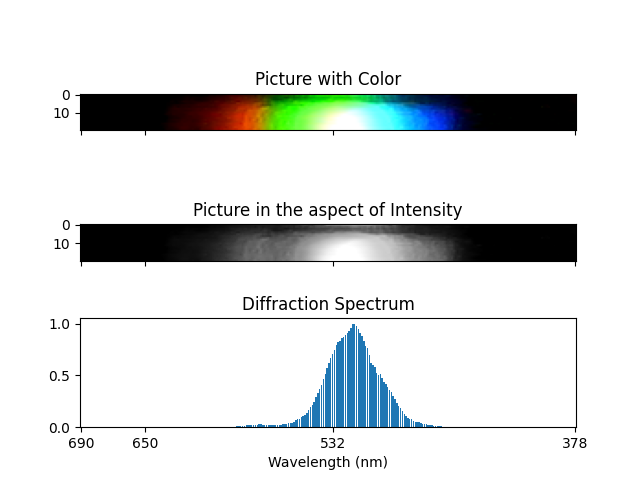
\includegraphics[width=4cm,height = 3cm]{绿色LED.png}}
\subfigure[蓝色LED]{
\label{Fig.sub.13}
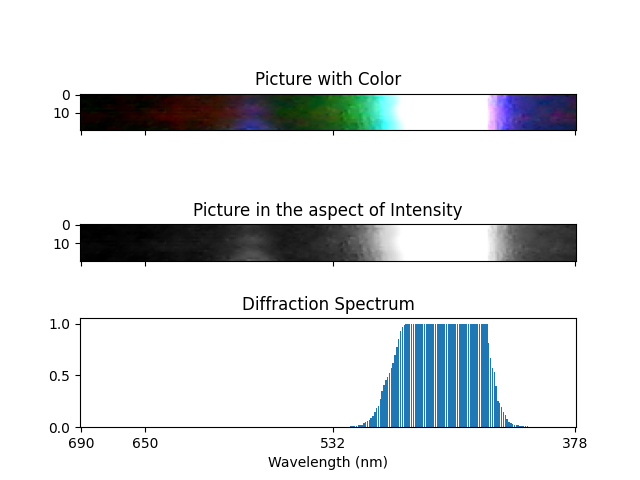
\includegraphics[width=4cm,height = 3cm]{纯蓝LED.png}}
\subfigure[黄色LED:可见是红加绿]{
\label{Fig.sub.14}
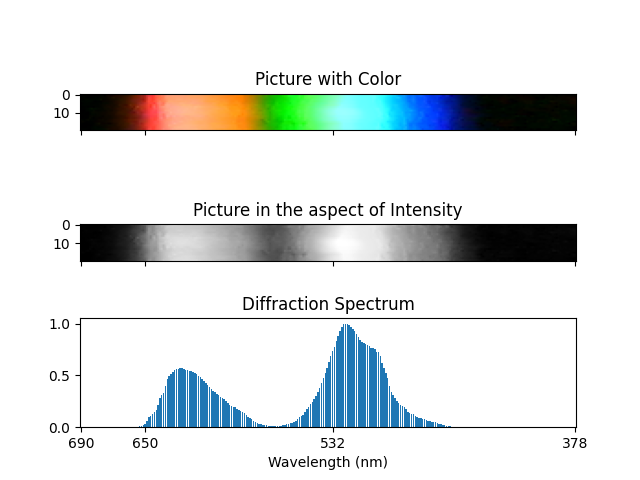
\includegraphics[width=4cm,height = 3cm]{黄色LED.png}}
\subfigure[浅蓝色LED:可见是绿加蓝]{
\label{Fig.sub.15}
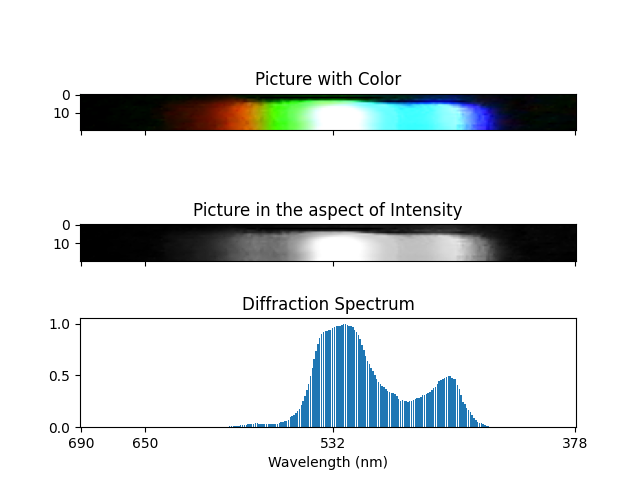
\includegraphics[width=4cm,height = 3cm]{浅蓝LED.png}}
\subfigure[粉紫色LED:可见是红加蓝]{
\label{Fig.sub.16}
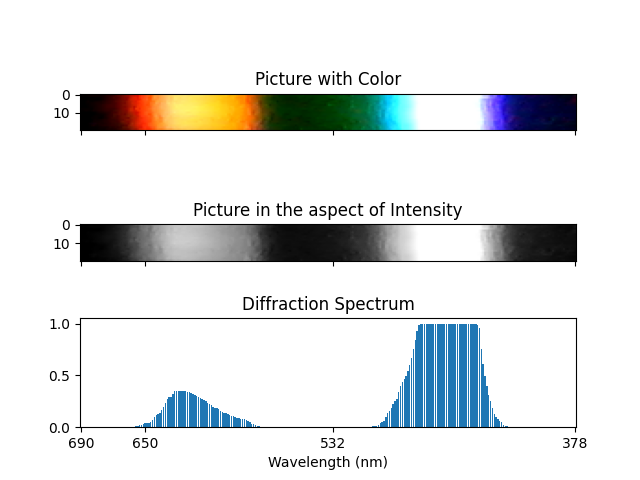
\includegraphics[width=4cm,height = 3cm]{粉紫色LED.png}}
\caption{不同颜色的LED}
\label{不同颜色的LED}


\end{figure}

\section{效果评价}
\subsection{缺点}
\begin{enumerate}
    \item 在结果显示上,只能够给出相对光强(用照片的灰度计算得到),而不能给出光强的准确值。这主要是因为我不知道相机镜头的内部参数,灰度值与实际物理光强的定量换算关系。
    \item 摄像机在CMOS质量不好,导致“噪音”较大。这一点在图\ref{Fig.sub.5}中反映得尤为明显。红色激光,对应位置的周围有较大“噪音”。我试图用算法减小“噪音”的干扰,但仍然不能够去除。
\end{enumerate}
\subsection{优点}
\begin{enumerate}
    \item 改进了光路,克服了相机作为光屏,存在\textbf{视角的问题}。\textbf{尽最大可能,接收各波段的衍射光。}
    \item 编写了程序:
    \begin{enumerate}
        \item 把众多操作集成在一个Python文件中,使得操作上非常便捷,\textbf{减少了重复劳动}和后期处理的难度。
        \item 程序中,给裁剪画面和激光校准设置了可调节的参数,使得这个程序对于不同机械机构的光谱仪(比如其他同学制作的),\textbf{可以采用同样的校准方法,迁移运用。}
    \end{enumerate}
    \item 将相机固定于光谱仪上,并用两束激光进行校准。\textbf{固定的机械结构和激光校准},使得位置$x$可以和波长$\lambda$建立准确的对应关系,大大\textbf{提高了测量精度。}
\end{enumerate}
\end{document}